
%%
%% MIT Thesis - Main Document
%%

\documentclass[12pt]{mitthesis}
\usepackage{lgrind}
\pagestyle{plain}

%\usepackage{thesis}
\usepackage[final]{graphicx}
\usepackage{amsmath,amsfonts,amssymb,amsthm}
\usepackage{verbatim}
\usepackage{color}
\usepackage{floatpag}
\usepackage{float}
\usepackage{listings} %code listing in API section
\lstset{basicstyle= \ttfamily}
\lstset{framesep=4pt}
\lstset{breaklines=true}
\usepackage{multirow}
\usepackage{epsfig}
\usepackage[section]{placeins}
%\usepackage{psfrag}
%\usepackage{makeidx}

%\usepackage[sort]{cite}
%\usepackage{citesort}
\usepackage[numbers,sort&compress,comma]{natbib}

\usepackage[draft=false,letterpaper,breaklinks,colorlinks,linktocpage,citecolor=blue,linkcolor=blue,urlcolor=blue]{hyperref}

% include parts of document
%\includeonly{titlepage,abstract,ack}

%%%%%%%%%%%%%%%%%%%%%%%%%%%%%%%%%%
%% PREAMBLE: Formatting and macros
%%%%%%%%%%%%%%%%%%%%%%%%%%%%%%%%%%

\typeout{}
\typeout{*****************************************************************************}
\typeout{Remember to do the following for LaTeX-ing of final document:}
\typeout{ * spell check .tex and .bib files}
\typeout{ * run BibTex and Index}
\typeout{ * check overfull hboxes}
\typeout{ * check table of contents and, if necessary, ...}
\typeout{ * increment toc page entry of Bibliography and Index}
\typeout{ * comment out the addcontentsline for Bibliography and Index}
\typeout{*****************************************************************************}
\typeout{}

% use footer to denote draft
%\cfoot{\scshape Draft: \today}

% no headers on full-page floats
\floatpagestyle{empty}

% create new float type for algorithm displays
\floatstyle{boxed}
\newfloat{algorithm}{tbh}{loa}
\floatname{algorithm}{Algorithm}
\newcommand{\algtop}{
  \vspace*{-6pt}
  \setlength{\belowdisplayskip}{2pt plus 2pt}
  \setlength{\abovedisplayskip}{2pt plus 2pt}
  \setlength{\itemsep}{4pt}
}
\newcommand{\algend}{
  \vspace*{-2pt}
}

\setlength{\leftmargini}{24pt} \setlength{\leftmarginii}{18pt}

% colors used in some figures
\definecolor{Black}{rgb}{0,0,0}
\definecolor{Blue}{rgb}{0,0,1.0}
\definecolor{Green}{rgb}{0,1.0,0}
\definecolor{Red}{rgb}{1.0,0,0}

\def\shortcite{\cite}

%\makeindex

\begin{document}

%%%%%%%%%%%%%%%
%% Front Matter
%%%%%%%%%%%%%%%

\include{cover}

\phantomsection
\addcontentsline{toc}{chapter}{Acknowledgments}

\chapter*{Acknowledgments}
\label{chap:ack}

This research is made possible with the help of many knowledgable people.
First, I would like to thank my advisor, Wojciech Matusik for many insightful suggestions and technical discussions
during the course of the project.
My collegues David I.W. Levin, Piotr Didyk, and Pitchaya Sitthi-Amorn have come up
with numerous great ideas and 
have helped with developing these ideas into practical solutions to the problems that I encounter.
Thanks to them for their creative minds and many hours of labor.
Thanks to my lab mates Kiril Vidim\v{c}e and Jonathan Ragan-Kelley for reading early drafts of this thesis and
providing valuable comments.
I would like to thank Hanspeter Pfister, Sylvain Paris, Fredo Durand and Ilya Baran for their helpful suggestions as well as Bernd Bickel, Moritz B\"{a}cher and  Milo\v{s} Ha\v{s}an for providing software and data.

Thank you to my father Mingda and my mother Yin for their constant support
and for inspiring me to conduct rigorous research.
Finally, I must thank Jiaqi, my best compannion for making my life a wonderful journey.


\setcounter{tocdepth}{3}
\tableofcontents
\cleardoublepage

\phantomsection
\addcontentsline{toc}{chapter}{List of Figures}
\listoffigures
\cleardoublepage

%\phantomsection
%\addcontentsline{toc}{chapter}{List of Algorithms}
%\listof{algorithm}{List of Algorithms}
%\cleardoublepage

%\phantomsection
%\addcontentsline{toc}{chapter}{List of Tables}
%\listoftables
%\cleardoublepage

%\phantomsection
%\addcontentsline{toc}{chapter}{Notational Conventions}
%\include{defn}
%\cleardoublepage

%%%%%%%%%%%%%%%%
%% Document Body
%%%%%%%%%%%%%%%%
\pagenumbering{arabic}
\renewcommand{\thepage}{\arabic{page}}
\setcounter{page}{1}
%%
%% MIT Thesis - Chapter 1
%%

%
\chapter{Introduction}
\label{chap:intro}
%
3D printing receives a lot of attention as it aims to democratize fabrication.
The ever expanding range of printing materials allows for fabrication of complex objects with spatially varying appearance, optical characteristics, and mechanical properties.
One of the most important unsolved problems in this area is how to compute an object's material composition from a functional or behavioral description. I will call this process \emph {specification to fabrication} translation (Spec2Fab). 
The goal of this work is to provide a convenient abstraction for specifying such translators. This is necessary to move past the current direct specification model of 3D printing.

Today,  3D printing of an object requires a material be directly specified for each voxel inside the object volume. This approach is fraught with difficulties. First, 3D printable models become specific to a single printer type, i.e., the models are built from materials provided by a given printer. Consider the inconvenience that would result from  word processing documents being compatible with specific 2D printers. Second, working directly with printing materials rather than material properties is extremely challenging for users. Imagine the difficulty in finding the right combination of printing materials that would provide a specific color, stiffness, or refractive index.

My work is motivated by the recent research efforts in the computer graphics community to create specific instances of the translation process, for example, subsurface scattering~\cite{Hasan:2010:PRO,Dong:2010:FSS} or deformation properties~\cite{Bickel:2010:DAF}. However, each of these instances is a custom, monolithic solution which is difficult to extend, combine, or modify. The main insight is that all these process instances share a similar structure. First, they rely on the ability to accurately simulate the physical properties of an object given its geometry and material assignment. They use this simulation within an optimization framework to search the space of all possible material assignments in order to find the one that best reproduces the desired properties. Due to the combinatorial nature of the search space the naive optimization approach is not tractable. For example, when the printing volume has $N$ voxels and each of these voxels can be assigned to one of $M$ base materials, the search space has $N^M$ dimensions. To overcome this problem, the search space is reduced to a lower-dimensional space using a reduction model. The goal of the reduction step is to aggressively shrink the search space in a domain-specific manner such that it still contains good approximations to the optimal solution. This search space reduction combined with the right choice of the optimization algorithm delivers a computationally tractable approximation.

The reduction-optimization structure suggests that it is possible to provide
a more general abstraction mechanism for translating 3D models to printer and material-specific representations.
This key observation leads to my thesis statement:

\emph{Spec2Fab processes share a similar structure and often use a small set of common components.}

I take the first step in building a unified model for Spec2Fab translation
and provide a small set of exemplar components as building blocks.
Towards this end, I propose two novel data structures designed to aid the fabrication process:
\begin{itemize}
\item The \emph{reducer tree} is a tree-based data structure that allows us to parameterize the space of material assignments.
\item The \emph{tuner network} is a data structure for specifying the optimization process.
\end{itemize}
My solution also provides an API for specifying the desired object, setting up the simulation, and defining parameters for the \emph{reducer tree} and \emph{tuner network}.
In general, my framework simplifies the construction of new computational fabrication algorithms.
More specifically, different components of the process can be easily replaced and other components easily reused. 
Various optimization strategies can also be explored with lower implementation burden. In order to show these advantages,
I illustrate how existing computational design processes fit into this framework and how they can be combined.
I demonstrate the results of these algorithms on a variety of different examples fabricated using 3D printers.

\include{RelatedWork}
\include{Overview}
\include{DataStructures}
\chapter{Process Configuration}
\label{sec:config}
In this section I show each step of process configuration. At the same time I describe my implementation of the 
\emph{reducer tree} and \emph{tuner network} data structures.

\section{Defining the Reducer Tree}
A \emph{reducer tree} can be constructed expediently using existing \emph{geometry} and \emph{material node} types.
\emph{Reducer trees} are not restricted to use only existing node types.
New node types can be added by extending the \verb|ReducerNode| class (see Figure~\ref{fig:node}).
In particular, implementing a new \emph{geometry node} type requires providing the function \verb|getOutputIndex|.
This function takes, as input, a 3D position and returns the \verb|id| of its child (Geometry or Material)
that contains this 3D point.
This function also computes a local coordinate for this child node.
Performing computations in local coordinates allows us to abstract away the geometry of a given object.
Implementing a new \verb|MaterialNode| type requires specifying the \verb|getMaterial| function
which takes a 3D point and returns the material at this point in the local geometry coordinate system.
Both types of nodes have an \verb|evaluate| function which is responsible for updating their internal states.
This function is used by the \emph{tuner network} to modify the internal state of the nodes.
As an example, we show a \emph{reducer tree} for performing texture mapping (see Figure~\ref{fig:red1}).
We also provide the corresponding pseudo-code (see Algorithm~\ref{alg:ReducerTree}).

\begin{figure}[h]
\centering
\includegraphics[width=0.6\linewidth]{figure/node.pdf}
\caption{Abstract interface for Node and its two subclasses.}
\label{fig:node}
\end{figure}

\begin{algorithm}
\caption{Constructing a \emph{reducer tree} for texturing}
\label{alg:ReducerTree}
\begin{lstlisting}[mathescape=true]
1. Create a root node $\mathbf{R}$ from inputMesh 
2. Subdivide $\mathbf{R}$ into outer layer $\mathbf{O}$ and inner volume $\mathbf{V}$ (Stratum Node) 
3. Subdivide $\mathbf{O}$ into set of columns $\mathbf{C}$ (Column Node) 
4. For each column $\mathbf{c}$ in $\mathbf{C}$ 
5.   Subdivide $\mathbf{c}$ into two layers (Layer Node) 
6. End 
\end{lstlisting}
\end{algorithm}

\section{Defining a \emph{Tuner}}
Recall that a \emph{tuner} consists of four components: a simulation, an error metric, an optimizer and a goal (\autoref{fig:tuner0}). Certain combinations of goal, metric and simulator are not compatible (i.e., a deformation simulator is not compatible with an error metric that compares images). Our API checks and prevents such incompatible combinations of components.  The optimization algorithm can request the error value for a given state using a callback function \verb|getError()| which is defined by the \emph{tuner}. Additional callback functions can be defined by the developer depending on the needs of the algorithm. For example, the branch and bound algorithm requires a custom  function to compute error bounds for a given state.

\section{Binding \emph{Tuners}}

\emph{Tuners} are assigned to nodes in the \emph{reducer tree} using the \verb|setNode| function. Once assigned, a \emph{tuner} can optimize the parameters of its associated subtree. \emph{Reducer nodes} provide a \verb|getSearchSpace| function which returns all free variables in the node subtree. In order to make \emph{tuners} as flexible as possible we provide a \verb|Parameter| class. Parameters can be either discrete or continuous, they can have associated bounds, and they can be marked as free or fixed.

\section{Establishing the \emph{Tuner Network}}

The \emph{tuner network} is an undirected graph that describes connections between \emph{tuners}. \emph{Tuner nodes} store a list of their neighbors. Only neighboring \emph{tuners} are allowed to exchange information. In our current implementation, this is accomplished using a shared memory array. As an example, we show how to construct and initialize a \emph{tuner network} for a simple optimization scheme -- a Simulated Annealing algorithm~\cite{Van:1987} (see Algorithm~\ref{alg:TunerNetwork}). The \emph{tuner network} also requires a schedule that specifies in what order individual \emph{tuners} should be executed. This schedule is specified by the developer. Once the \emph{tuner network} is constructed, the process configuration phase is complete. We obtain a compiled executable that computes desired material assignment from an input specification.
\begin{algorithm}
\caption{Connecting and executing the \emph{tuner network}}
\label{alg:TunerNetwork}
\begin{lstlisting}[mathescape=true]
1.  for each Tuner $\mathbf{T}_i$ attached to a plane
2.    for each Tuner $\mathbf{T}_j$ adjacent to $\mathbf{T}_i$
3.      add $\mathbf{T}_j$ to $\mathbf{T}_i$'s list of neighbors
4.    end
5.  end
6.  iterate N times
7.  for each Tuner $\mathbf{T}_i$
8.    set temperature for $\mathbf{T}_i$'s optimizer
9.    run $\mathbf{T}_i$
10. end
\end{lstlisting}
\end{algorithm} 
\section{Process Use}
\label{sec:use}
The compiled program, which executes the \emph{tuner network}, takes five types of arguments: the input geometry, the goal, the simulation configuration, a set of materials and the target 3D printer specification. 
After the \emph{tuner network} is executed, the parameters of the \emph{reducer nodes} in the \emph{reducer tree} are set. It is then straightforward to compute the material assignment at arbitrary resolution. Since, a typical multi-material 3D printer requires a volumetric model with per voxel material assignment, we can simply iterate over all voxels in the volume. We obtain the material assignment by evaluating (\verb|getMaterial|) of the \emph{reducer tree} root at the center of each voxel location. This representation can be easily converted to a printer specific format for output. For the Objet500 Connex printer used in this paper we extract material isosurfaces which are submitted to the printer as STL files. 
\chapter{Experiments}
\label{chap:results}
\biglet{I}{n} order to evaluate capabilities of our system, I have implemented a number of existing translation processes.
Furthermore, the ease with which different algorithm components can be combined enables the creation of two new translation processes.
The first combination is an algorithm that can produce objects with desired refractive properties and an associated texture.
The second algorithm applies a desired texture to an object with prescribed deformation behavior.
All of these processes, both from prior work and new ones, should easily fit into our framework. I printed the objects using a Stratasys Object500 Connex  multi-material printer.
The following paragraphs provide a detailed description of how the individual algorithms can be designed with my system.
%All \emph{reducer trees} and the \emph{tuner networks} for producing these results are presented in 
%\autoref{fig:ReducerTreesAdditional}.

\section{Spatially-varying Albedo}
I have designed a Spec2Fab translator that allows 3D printing of textured models (Figure~\ref{fig:textured}).
The \emph{reducer trees} and the \emph{tuner networks} for producing these results are presented in 
\autoref{fig:treeTexture}.
Being able to apply precisely specified spatially-varying albedo values to printed models is a crucial capability.
However, no standard processes have been designed for this task so far.
The input to the texturing algorithm is a shape and its desired albedo texture.
Since the texture is only affected by materials close to the surface,
I use a \emph{stratum node} to divide the input shape into a thin shell and an inner volume.
I then divide the outer layer into columns.
The set of printable colors is expanded by stacking translucent materials using the \verb|LayeredMaterial| Node.
The number of layers is fixed to the number of print materials.
The reduced parameters are the thickness values of each material layer.
For each column, the \emph{tuner}'s optimizer looks up the proper stacking that produces the closest albedo value.
Due to printer resolution, the range of albedo values that can be achieved is quantized.
I therefore implement an error diffusion algorithm by connecting neighboring \emph{tuners}.
In this simple algorithm, the simulation is a table lookup using measured albedo value corresponding to different base materials.

\begin{figure*}[t]
\centering
\includegraphics[width=0.95\linewidth]{figure/texture.pdf}
\caption {The reducer-tuner model enables creating objects of arbitrary shapes with embedded textures.}
\label{fig:textured}
\end{figure*}

\begin{figure*}[t]
\centering
\includegraphics*[scale=0.7]{figure/treeTexture.pdf}
\caption{\emph{Reducer tree} for texture.}
\label{fig:treeTexture}
\end{figure*}

\section{Heterogeneous Subsurface Scattering}
I have replicated the subsurface scattering process of Ha\v{s}an et al.~\shortcite{Hasan:2010:PRO} using a tree
shown in Figure~\ref{fig:treeSubs}. A 3D printed chessboard is shown in Figure~\ref{fig:sub}.
The input to this algorithm is a 3D mesh along with subsurface-scattering profiles defined
at a set of surface points.
We use the same \emph{reducer tree} as in the texture example thereby simplifying the process configuration phase.
Since the \emph{reducer tree} adapts to the input geometry, I can apply the same marble material to arbitrary
meshes such as the dome shown in Figure~\ref{fig:dome}.
The only difference is that I allow each column to have four layers of varying thickness and material.
I use a branch and bound optimization algorithm which has been modified to handle continuous parameters by allowing discrete increments.
I implement a bound estimate callback function specific to this problem.
Each column is optimized independently using the algorithm. 
The simulation computes a scattering profile for a given stacking
and the error metric compares the simulated and goal profiles using squared error.
\begin{figure}[h]
\centering
\includegraphics[scale=0.7]{figure/treeSubs.pdf}
\caption{
	\emph{Reducer tree} for heterogeneous subsurface scattering effect.}
\label{fig:treeSubs}
\end{figure}

\begin{figure}[h]
\centering
\includegraphics[width=0.65\linewidth]{figure/fig_chess.pdf}
\caption{
	A marble chessboard with prescribed subsurface scattering properties produced by Ha\v{s}an et al.~\shortcite{Hasan:2010:PRO}.
	The insets show the samples under thin line illumination, and the graph shows the convergence of tuners for 10 out of 100 scattering profiles used in the example. The error is measured by square distance between two profiles, each containing 400 coefficients.}
\label{fig:sub}
\end{figure}

\begin{figure}[h]
\centering
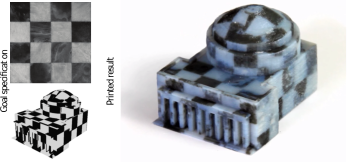
\includegraphics[width=0.45\linewidth]{figure/dome.png}
\caption{
	A marble dome produced by the subsurface scattering \emph{reducer tree}.}
\label{fig:dome}
\end{figure}

\section{Goal-based Caustics:}
I have configured two different processes for computing goal-based caustics (Figure~\ref{fig:caust}). While they define exactly the same goal, they have very different \emph{reducer trees} and \emph{tuner networks}.
The first process is based on the work of Papas et al.~\shortcite{Marios:2011}.
It computes a set of micro-lenses which produce the desired caustic image as shown in Figure~\ref{fig:facet}.
The image is pre-processed into a set of Gaussian distributions.
Each distribution is matched with a microlens.
The optimization applies simulated annealing to permute the location of these micro-lenses
in order to construct a smooth surface.
The micro-lenses are represented using \emph{plane nodes}.
The complete reducer tree is shown in Figure~\ref{fig:treeFacet}.
In the \emph{tuner network}, each \emph{tuner} is connected to its four neighbors.
During the execution of an individual \emph{tuner},
the optimization algorithm makes a randomized decision
about whether or not to swap its micro-lens with one of its neighbors based on smoothness of the surface.
The \emph{tuners} are executed many times until a user-specified convergence criterion is met. 

\begin{figure}
\centering
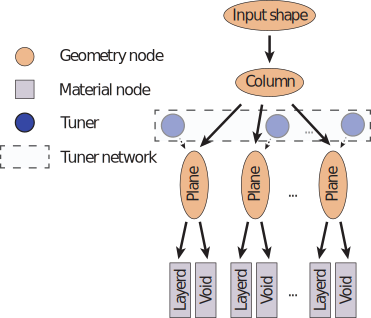
\includegraphics[scale=0.7]{figure/treeFacet.pdf}
\caption {\emph{Reducer tree} for facet caustics.
}
\label{fig:treeFacet}
\end{figure}

\begin{figure}
\centering
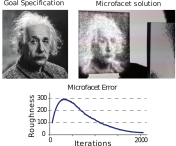
\includegraphics[width=0.65\textwidth]{figure/facet.pdf}
\caption {3D printed lens arrays that produce a caustic image of Einstein.
The algorithm is proposed by Papas et al.~\shortcite{Marios:2011}.
Below we show convergence plots for the microfacet optimizations.
The portrait is available from the United States Library of Congress's Prints and Photographs division,
now in the public domain.
}
\label{fig:facet}
\end{figure}

The second process is based on the work of Finckh et al.~\shortcite{Finckh:2010} (Figure~\ref{fig:spline}).
I use a \emph{B-spline node} to represent a smooth surface.
This is in contrast to the potentially discontinuous surface in the method above.
The reduced parameters are the height of each spline control point.
I implement a simple caustics simulator for height fields.
The simulated image is compared to the goal image using mean squared error.

\begin{figure}
\centering
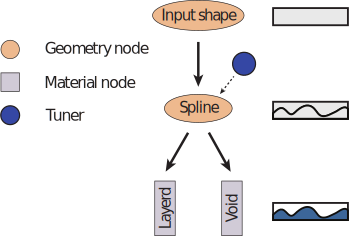
\includegraphics[scale=0.7]{figure/treeSpline.pdf}
\caption {\emph{Reducer tree} for smooth caustics.
}
\label{fig:treeSpline}
\end{figure}

\begin{figure}
\centering
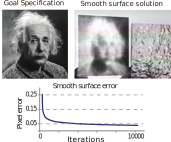
\includegraphics[width=0.65\textwidth]{figure/spline.pdf}
\caption {A smooth surface that produces a caustic image of Einstein.
The algorithm is proposed by Finckh et al.~\shortcite{Finckh:2010}.
Below we show convergence plots for the smooth surface optimization.
}
\label{fig:spline}
\end{figure}

\section{Elastic Behavior:}
In the spirit of Bickel et al.~\shortcite{Bickel:2009},
I have implemented an algorithm to compute material distribution based on a desired force-displacement response.
The input to this algorithm is a mesh, a simulation configuration, and a desired shape.
Simulation configuration includes vertex constraints and forces applied to the mesh.
For this example, I use a co-rotational finite element method (FEM) simulation
with linearly elastic materials to estimate the objects deformation.
For the \emph{reducer tree}, I use a voxel partition to divide the object into a low-resolution grid.
I assign a single material to each grid cell.
The FEM simulator queries the \emph{reducer tree} for material assignments at arbitrary spatial locations.
I use the same branch and bound algorithm as in our subsurface-scattering process
but with a different bound computation callback function.
I use the mean squared distance between the simulated and the desired shapes as the error metric.
I have designed a simple experiment to validate this process
in which I set the goal of our optimization to be a given deformed state (\autoref{fig:book}).

\begin{figure}
\centering
\includegraphics[width=0.65\linewidth]{figure/fig_sub.pdf}
\caption {A 3D printed book with prescribed deformation behavior under load.
The plot shows the error (in meters) as a function of iteration number of our branch and bound based \emph{tuner}.
The blue line shows the smallest error seen so far while the red line the \emph{tuner}'s progress exploring material subtrees~\protect\cite{Bickel:2009}.}
\label{fig:book}
\end{figure}

\section{Combining Caustics and Spatially-varying Albedo:}
The first of my new combined translation processes incorporates both smooth caustics and texture mapping.
More specifically, I will compute a transparent slab with a texture image that, when illuminated, casts a prescribed caustic image.
The input slab is split into two pieces using a \emph{plane node} as shown in Figure~\ref{fig:ReducerTreesAdditional}.
The top piece is tuned to produce an input image. The material in the top piece is then fixed. The bottom piece is then tuned to produce a caustics image.


\section{Combining Deformable Object and Spatially-varying Albedo:}
My second new process combines spatially-varying albedo and elastic deformation properties.
This is a very useful combination since when modeling objects we would like to specify both their appearance and ``feel''.
In this process, the input shape is divided into a thin shell and an inner volume.
I will optimize for the deformation behavior and the texture independently due to the limitations of our current FEM simulator.
As the outer shell is very thin, it has negligible influence on overall object deformation.

\begin{figure*}[t]
\centering
\includegraphics*[clip, width = \linewidth]{figure/ReducerNetworksSuplemental}
\caption{The figure shows all \emph{reducer trees} proposed in this proposal.
\textbf{Smooth caustics:} The smooth caustics tree consists of a spline surface that divides the geometry into an inner surface filled with a transparent material and an outer, void surface. Void material can be used to implement displacement mapping.
Here, a single \emph{tuner} can be used ti deform the spline surface.
\textbf{Smooth caustics/texture:} The smooth caustics/texture \emph{reducer tree} splits the object into upper and lower sections using a plane.
The upper section then uses the Smooth caustics \emph{reducer tree} to define surface displacements while the lower section uses a set of columns as texture pixels.
Here, a single \emph{tuner} solves for the caustic image and a set of \emph{tuners} with regular connectivity solves for the textured image.
\textbf{Deformation/texture:} The object is divided into an outer layer and inner volume using a stratum node.
The interior volume is then voxelized and each voxel is assigned a layered material.
As in the previous example, the outer layer is divided into columns which are used as pixels for the texture image.
The \emph{tuner} setup is also similar to the previous example except the single \emph{tuner} is used to optimize the mechanical behavior of the object.
\textbf{Facet caustics:} Here, I will build facets by dividing an object into columns and then bisecting the columns horizontally with a plane.
The orientation of this plane defines the angle of the facet surface. 
I will use a \emph{tuner network} to optimize for smooth plane orientations.
\textbf{Subsurface scattering/texture:} The subsurface scattering/texture \emph{reducer tree} partitions the object into an inner volume and outer layer using a \emph{stratum node}.
The inner volume is unimportant in this example so I  can place a constant material there.
The outer material is divided into pixels using the \emph{column node}.
These columns are filled with layered materials.
I can optimize each column separately using an associated \emph{tuner}.}
\label{fig:ReducerTreesAdditional}
\end{figure*}

\chapter{Discussion}
\biglet{T}{hrough} the above series of experiments, I will confirm whether \emph{reducer tree} and \emph{tuner network} can allow us to reuse a large number of software components.
In the extreme case, the subsurface scattering algorithm can be obtained by trivially adapting the same \emph{reducer tree} for texture mapping objects.
The power of component reuse is further elucidated by the presence of \emph{column nodes} in most examples and by the reuse of optimization schemes (such as branch and bound) in multiple algorithms.
The \emph{reducer tree} and \emph{tuner network} will make these similarities easy to observe and exploit.
The only component whose reusability was not demonstrated in this proposal is simulation.
In this work, I will aim to fabricate objects with a wide range of physical properties and this necessitates the use of a wide range of simulation algorithms. Finally, once a whole process is configured, it is independent of input geometry and goal parameters. For example, I can run the spatially-varying albedo process with different geometries and input textures

The \emph{reducer-tuner model} is ideally suited for multi-material printing capable of producing objects with a wide range of different properties.
In order to showcase these strengths, I will fabricated my examples for an Objet500 Connex -- a phase change inkjet printer that uses photopolymers with a wide range of optical and mechanical properties. Even though only two materials can be used and mixed within a single object, our framework has been proven to be very useful. 
As the number of materials that can be printed simultaneously will grow, we expect the methodology presented here to increase in utility.
For other types of 3D printing technologies, Spec2Fab framework has a reduced use. In the case of 3D printing using a single, rigid material (e.g., fused filament fabrication or Stereolithography) the framework can be used to tune geometry of objects. For plaster-based 3D printers that produce full-color 3D prints, Spec2Fab framework can be employed to compute proper texturing of objects.

\include{Conclusion}

%%%%%%%%%%%%%%
%% Back Matter
%%%%%%%%%%%%%%

% appendixes
\appendix
%\include{appendix1} % appendix1.tex should be in the same directory in this case
%\include{appendix2} % appendix2.tex should be in the same directory in this case

% bibliography
\cleardoublepage
\phantomsection
\addcontentsline{toc}{chapter}{Bibliography}
%\bibliographystyle{plain}
\bibliographystyle{plainnat}
\bibliography{paper} % use with BibTeX (bibliography.bib should be in the same directory in this case)

% index (uncomment the lines below if you want an index)
%\newpage
%\mbox{}
%\newpage
%\addcontentsline{toc}{chapter}{Index}
%\printindex

\end{document}
